\chapter{Componenti del Progetto}\label{ch:chapter2}
TUTTE LE INFORMAZIONI LE HO PRESE DA WIKIPEDDIA E DAI DOCS DI PYTORCH
\section{PyTorch}
\textbf{PyTorch} è una libreria di \textit{Machine Learning} open source basata sulla libreria \textbf{Torch}, utilizzata per applicazioni come la visione artificiale e l'elaborazione del linguaggio naturale, sviluppata principalmente dal laboratorio di ricerca AI di Facebook.È un software gratuito e open source nato  per essere utilizzato con il linguaggio di Programmazione Python(come avviene in Questo Elaborato), PyTorch ha anche un'interfaccia C ++.
Ho utilizzato questa librearia perchè fornisce due specifiche molto utili per lavorare con le Reti Neurali:\textit{Pytorch Tensor} e i Moduli (AutoGrad ,Optim, nn).
PyTorch definisce una classe chiamata Tensor (torch.Tensor) per memorizzare e operare su array di numeri rettangolari multidimensionali omogenei.
\newpage
\subsection{PyTorch Tensor}
I tensori PyTorch sono simili agli array NumPy, ma possono essere utilizzati anche su una GPU Nvidia compatibile con CUDA. Per Lavorare al \textbf{Visual Recognition} è molto utile lavorare su GPU: I tempi e le perfomance ne risentono in positivo.
\subsection{Moduli}
PyTorch utilizza un metodo chiamato \textit{automatic differentiation}(\textbf{AutoGrad Module}). Un \textit{Recorder} registra le operazioni eseguite, quindi le riproduce all'indietro per calcolare i gradienti. Questo metodo è particolarmente potente quando si costruiscono reti neurali per risparmiare tempo in un'epoca calcolando la differenziazione dei parametri nel passo del \textit{Forward}.
\newline
Il secondo Modulo che ci interssa è \textbf{Optim Module}(\textit{torch.optim}).
È un modulo che implementa vari algoritmi di ottimizzazione utilizzati per la creazione di reti neurali. La maggior parte dei metodi più utilizzati sono già supportati, quindi non è necessario crearli da zero. In particolare l'algortimo di Ottimizzazione che ho utilizzato in questo elaborato è \textit{optim.Adam} il quale implementa lo stochastic gradient descent.
Durante il Training si utilizzeranno i metodi della classe optim come \textit{ .zero\_grad()} e successivamente \textit{.step()} per fare l'update dei parametri della rete.
\newline
Infine Abbiamo il Modulo \textbf{\textit{torch.nn}} che ci fornisce molte più classi  per implementare e addestrare la \textit{Rete Neurale}. In particolare ci aiuta nella definizione della \textit{Rete Neurale}, e in quella dei layers che la formano.
\newpage
I Package utilizzati in questo elaborato sono:
\begin{itemize}
    \item \textit{torch.nn.Module}: È una classe base per tutti i moduli di \textit{Rete Neurale}
    \item \textit{torch.nn.Linear}: utilizzato per i layer \textit{Fully Connected}
    \item \textit{torch.nn.Conv2d}:utilizzato per i \textit{Layer Convoluzionali}
    \item \textit{torch.nn.MaxPool2d}:Viene utilizzato per applicare un max pooling 2D 
    \item \textit{torch.nn.ReLU}:Funzione di attivazione dei layer
    \item \textit{torch.nn.CrossEntropyLoss}: funzione per il calcolo della \textit{Loss} della Rete
\end{itemize}
\section{Dataset} 
\subsection{CIFAR-10}
Il Dataset utilizzato in questo elebaorato è \textbf{CIFAR-10}.
Il Dataset \textbf{CIFAR-10} è costituito da 60000 immagini a colori (avranno 3 canali per ciascuna immagine per gestire l'RGB) 32x32 divise in 10 classi, con 6000 immagini per classe. Sono disponibili 50000 immagini di allenamento e 10000 immagini di prova.\newline
Il Dataset è suddiviso in cinque batch di Training e un batch di Testing, ciascuno con 10000 immagini. Il batch di prova contiene esattamente 1000 immagini selezionate casualmente da ciascuna classe. I batch di Training contengono le immagini rimanenti in ordine casuale, ma alcuni di essi possono contenere più immagini di una classe rispetto a un'altra. In  particolare, i batch di Training contengono esattamente 5000 immagini di ciascuna classe.
\newpage
In questa immagine possiamo notare le dieci Classi di \textbf{CIFAR-10} oltre a diei esempi presi in maneira casuale da ciascuna classe.
\begin{figure}[ht]
\centering
\caption{Classi di CIFAR-10}
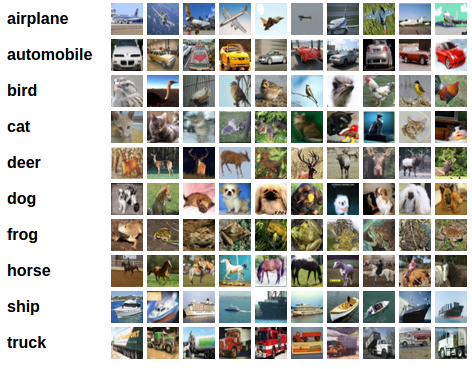
\includegraphics[width=\linewidth]{CIFAR.png}
\label{figure : CIFAR-10}
\end{figure}

\subsection{Gestione del Dataset}
Alla base della gestione dei \textit{Dataset} vi è la classe \textit{torch.utils.data.DataLoader}.
In Particolare tutti  sono sottoclassi di torch.utils.data.Dataset, ovvero hanno implementati i metodi \textit{getitem()} e \textit{len()}.
\newline
Per gestire il Dataset \textbf{CIFAR-10} ho istanziato nel mio progetto una classe \textit{Filtered\_dataset} che si occcupasse di questa mansione.
L'obbiettivo del mio elaborato era rappresentare il problema del \textbf{Continual Learning} e per fare ciò è necessario dividere il dataset utilizzato in \textit{Tasks}.
Ciò significa che a seconda del numero di \textit{Tasks} che io voglio utilizzare per simulare il \textbf{Continual Learning}
dovrò dividere il Dataset per \textit{Label}. Ad Esempio se io volessi utilizzare 5 \textit{Tasks}, per ognuno di essi avrei 2 \textit{Label}.\newline
La classe \textit{Filtered\_dataset} si occupa di creare un Subset con con il metodo della libreria di \textbf{PyTorch} \textit{torch.utils.data.Subset} che crea un subset del Dataset originario.\newline
Nel processo di suddivisione del Dataset è stato necessario \textit{mappare} le labels del dataset in modo tale da essere coerenti con l'output dell Rete. In particolare ciò è stato fatto tramite due attributi della classe \textit{Filtered\_dataset}:\textit{original2task} e \textit{task2original}. Questi due attributi consistono in due dizionari con chiave-valore le label e la rispettiva mappatura.
Ho reso inlotre possibile \textit{randomizzare} le label all'interno di ciascun task per poter fare ulteriori test con il metodo \textit{idx\_tasks}.
\newline
\section{Rete Neurale Convoluzionale}
La \textbf{Rete neurale Convoluzionale} (CNN o ConvNet) è una classe di \textit{Reti Neurali} profonde, molto spesso  applicata all'analisi ed al riconoscimento delle immagini.
La \textbf{Rete neurale Convoluzionale} che ho utilizzato in questo progetto è formata da sei \textit{Conv2D} layers separati da due \textit{MaxPool2D} ed infine da due \textit{Fully Connected Layer} sui cui ho applicato \textit{Dropout} per limitare l'\textit{Overfitting} durante il Training.
\newline
La particolarità di questa rete è che il layer dell'output è \textbf{\textit{Dinamico}}, cioè che cambia a seconda del numero di \textit{tasks} su cui si vuole lavorare e sulla tipologia di approccio scelto tra \textit{Task-Agnostic} e \textit{Task-Aware}.\newline
In Particolare è possibile aggiungere nuovi layer di output con il metodo\textit{add\_task} che richiama semplicemnte il metodo \textit{add\_module} della classe \textit{nn.Module}.
Un altro metodo importante della \textit{Rete Neurale} sarà  \textit{set\_tasks} che mi permette di settare il numero di tasks che voglio avere come output. I due attributi fondamentali della classe \textit{net} sono \textit{task\_fcs} e \textit{current\_tasks}, che sono sostanzialmente due Array contenenti gli indici dei \textit{tasks}. Il primo conterrà tutti i layer lineari per le varie  \textit{Classification Head}, mentre il secondo, seleziona quale(i) task(s) sono correntemente attivi.
Qui di seguito riporto la \textit{Rete Neurale} per un singolo task con tutte le classi corrispondente al \textit{Joint Training}:

\newline
Net(\\
  (conv1): Conv2d(3, 32, kernel_size=(3, 3), stride=(1, 1), padding=(1, 1))\\
  (conv2): Conv2d(32, 64, kernel_size=(3, 3), stride=(1, 1), padding=(1, 1))\\
  (conv3): Conv2d(64, 64, kernel_size=(3, 3), stride=(1, 1), padding=(1, 1))\\
  (pool): MaxPool2d(kernel_size=2, stride=2, padding=0, dilation=1, ceil_mode=False)\\
  (conv4): Conv2d(64, 128, kernel_size=(3, 3), stride=(1, 1), padding=(1, 1))\\
  (conv5): Conv2d(128, 128, kernel_size=(3, 3), stride=(1, 1), padding=(1, 1))\\
  (conv6): Conv2d(128, 256, kernel_size=(3, 3), stride=(1, 1), padding=(1, 1))\\
  (fc1): Linear(in_features=16384, out_features=120, bias=True)\\
  (fc2): Linear(in_features=120, out_features=84, bias=True)\\
  (dropout): Dropout(p=0.5, inplace=False)\\
  (task0\_fc): Linear(in_features=84, out_features=10, bias=True)\\
)
\newpage
Il layer \textit{Task0\_fc} è l'ultimo layer che è stato aggiunto con \textit{add\_task} e \textit{settato} con \textit{set\_task}.
Se l'esperimento fosse stato condotto su più \textit{Tasks} ci sarebbero stati altri layers oltre a \textit{Task0\_fc}. Nel caso in cui l'output voluto fosse stato su più tasks, nel metodo \textit{Forward} della rete tramite \textit{torch.cat}, sarebbero stati concatenati tra di loro i parametri corrispondenti selezionati da \textit{current\_tasks}.
\newline
La \textit{funzione di Attivazione} utilizzata nei layer \textit{Convoluzionali} è \textbf{ReLu}, come anticipato precedentemente.
La \textbf{rectified linear activation function} o \textbf{ReLU} in breve è una funzione lineare a tratti che darà  come output direttamente l'input se è positivo, altrimenti produrrà zero. L'utilizzo della \textbf{ReLu} consente di ottenere un \textit{Training} e una performance migliori.
\newline
Per quanto riguarda la funzione che si occupa del calcolo della \textit{Loss} ho optato per utilizzare la \textbf{CrossEntropyLoss}. Questa Funzione combina in una unica classe \textit{nn.LogSoftmax()} e \textit{ nn.NLLLoss()}.
Come anticipato nel paragrafo relativo a \textbf{PyTorch} ho utilizzato come \textit{optimizer} \textbf{SGD} con \textit{Learning Rate} pari a  \mathbf{0.001}.\newline
Infine, ho reputato necessario applicare \textbf{Dropout} ai due \textit{Fully Connected Layer} che precedono il layer di output dinamico. Durante il \textit{Training}, azzera in modo casuale alcuni degli elementi del tensore di input con probabilità p utilizzando campioni da una distribuzione di Bernoulli. In questo modo ho diminuito L'\textit{Overfitting}  riscontrato sulla \textit{Rete}.